\chapter{Cooperation}\label{ch:cooperation}
\begin{chapter_outline}

This chapter covers the required basics and related works in the cooperative setting.
After an introduction in Section~\ref{sec:ch3_intro}, we define in Section~\ref{sec:ch3_decpomdp} the cooperative framework called decentralised partially observable Markov decision process.
Section~\ref{sec:ch3_env} presents examples of its application, followed by a precise description of the StarCraft multi-agent challenge, a popular environment suite in this manuscript.
We then detail several value-based methods in Section~\ref{sec:ch3_value} and policy-based methods in Section~\ref{sec:ch3_policy}.
We finally discuss other approaches of interest in Section \ref{sec:ch3_further}.
\end{chapter_outline}

\section{Introduction}
\label{sec:ch3_intro}
As introduced in Part~\ref{part:background}, cooperation is the multi-agent setting of agents sharing a common goal.
This second part of the thesis considers the decentralised POMDP (Dec-POMDP)~\citep{DecPomdp}, a framework where all agents receive the same reward.
Such a framework is also called common reward games, e.g. by~\cite{marl-book}.
Its definition is provided in Section~\ref{sec:ch3_decpomdp}.

Nevertheless, when it comes to cooperation in a multi-agent system, one topic to discuss is whether action selection and agent training are centralised or decentralised.
This is also referred to as the modes of execution and training in~\citep{marl-book}.
This manuscript considers three combinations: centralised training and execution, decentralised training and execution, and centralised training with decentralised execution.

Since all agents receive the same reward, training a single agent that centrally selects joint actions is possible and would benefit from sharing common knowledge.
This is the centralised mode, where one agent is trained with SARL methods.
For example, controlling a robotic hand composed of several actuators can be done with a single agent controlling every actuator.
However, as presented in Section~\ref{sec:ch2_partial_observability}, some setting induces partial observability.
All agents may not access the same information or perceive only a part of the environment's state.
It would then be impossible to consider that one agent can replace all agents and select actions in a centralised mode.

On the contrary, the decentralised execution mode considers that each agent selects its action independently.
This can be done irrespective of the information they can access.
The corresponding decentralised training mode is when these agents are trained independently.
In other words, these agents assume they are the single agent learning in the environment.
We refer to the decentralised mode when training agents independently with SARL to select an action based on their observation.

Finally, the third mode unifies the two formers and is centralised training with decentralised execution (CTDE).
It allows decentralised execution, with each agent selecting actions based on their observations, but allows for the exploitation of more information during training.
Indeed, RL agents are usually trained in a simulator, having access to every piece of information.
Typically, this mode benefits from the state of the environment or exploits the actions made by other agents during training.

From the research question highlighted in Chapter \ref{ch:introduction}, these different modes showcase several ways to consider, or not, the other learning agents when training one.
This Part~\ref{part:coop} focuses on methods that exploit the CTDE mode to solve cooperative tasks.
This chapter presents Dec-POMDP environments and CTDE methods issued from the literature.
The performance of these methods is not compared in this chapter but in both next ones.
They present two specific contributions: another CTDE method in Chapter~\ref{ch:qvmix} and a real-world application of Dec-POMDP in Chapter~\ref{ch:impmarl}.

\section{Decentralised partially observable Markov decision process}
\label{sec:ch3_decpomdp}
As introduced, the definition of the decentralised partially observable Markov decision process (Dec-POMDP)~\citep{DecPomdp} can be derived from the partially observable stochastic game definition.
It is the same, except the reward function maps to a single reward common to all agents.

We define the Dec-POMDP by a tuple $[\mathcal{S}, \mathcal{Z}, \mathcal{U}, n, O, R, P, \gamma, T, p]$, where $n$ agents $a_i$, $i \in \mathcal{A} \equiv \{1,..,n\}$, simultaneously choose an action at every time step $t$.
The interaction of the agents with the environment in a Dec-POMDP is presented in Figure \ref{fig:ch3_decpomdp}.
The state of the environment is $s_t \in \mathcal{S}$ where $\mathcal{S}$ is the set of states.
The observation function $O:\mathcal{S} \times \mathcal{A} \rightarrow \Delta(\mathcal{Z})$ maps the state to the probability of agent $a$ to perceive the observation $o_t^{a} \in \mathcal{Z}$ at time $t$, where $\mathcal{Z}$ is the observation space.
Each agent selects an action $u_t^{a} \in \mathcal{U}^{a}$ based on its policy $\pi^{a}(u_t^{a}|\tau_t^{a},o_t^{a}): (\mathcal{Z} \times \mathcal{U}^a)^t \times \mathcal{Z}\rightarrow \Delta(\mathcal{U}^a)$, which maps its history $\tau_t^{a} \in (\mathcal{Z} \times \mathcal{U}^a)^{t-1}$ and its observation $o_t^{a}$ to the probability of taking action $u_t^{a}$. 
The joint action space is $\mathcal{U} \equiv \bigtimes_{i \in \mathcal{A}} \mathcal{U}^{a_i}$ and the joint or team policy is denoted by $\mathbf{\pi}=(\pi^{a_1},...,\pi^{a_1})$.
After the joint action $\mathbf{u_t} \in \mathcal{U}$ is executed, the transition function determines the new state with probability $P(s_{t+1}|s_t, \mathbf{u_t}): \mathcal{S} \times\mathcal{U} \rightarrow  \Delta(\mathcal{S}) $, and $r_t=R(s_{t+1}, s_t, \mathbf{u_t}): \mathcal{S} \times \mathcal{S} \times \mathcal{U} \rightarrow \mathbb{R}$ is the team reward obtained by all agents.
The goal of agents is to find their optimal policy that maximises the expected return during the entire episode of T time step $\mathbb{E}[G_0|\mathbf{\pi}, p]$ where $G_0=\sum_{t=0}^{T-1} \gamma^{t} r_{t}$ and $p$ is the initial state distribution.
The optimal joint policy is denoted by $\mathbf{\pi^{*}} =\argmax_{\mathbf{\pi}} \mathbb{E}[G_0|\mathbf{\pi}, p]$, achieved if all agents plays the optimal policy.

\begin{figure}
    \centering
    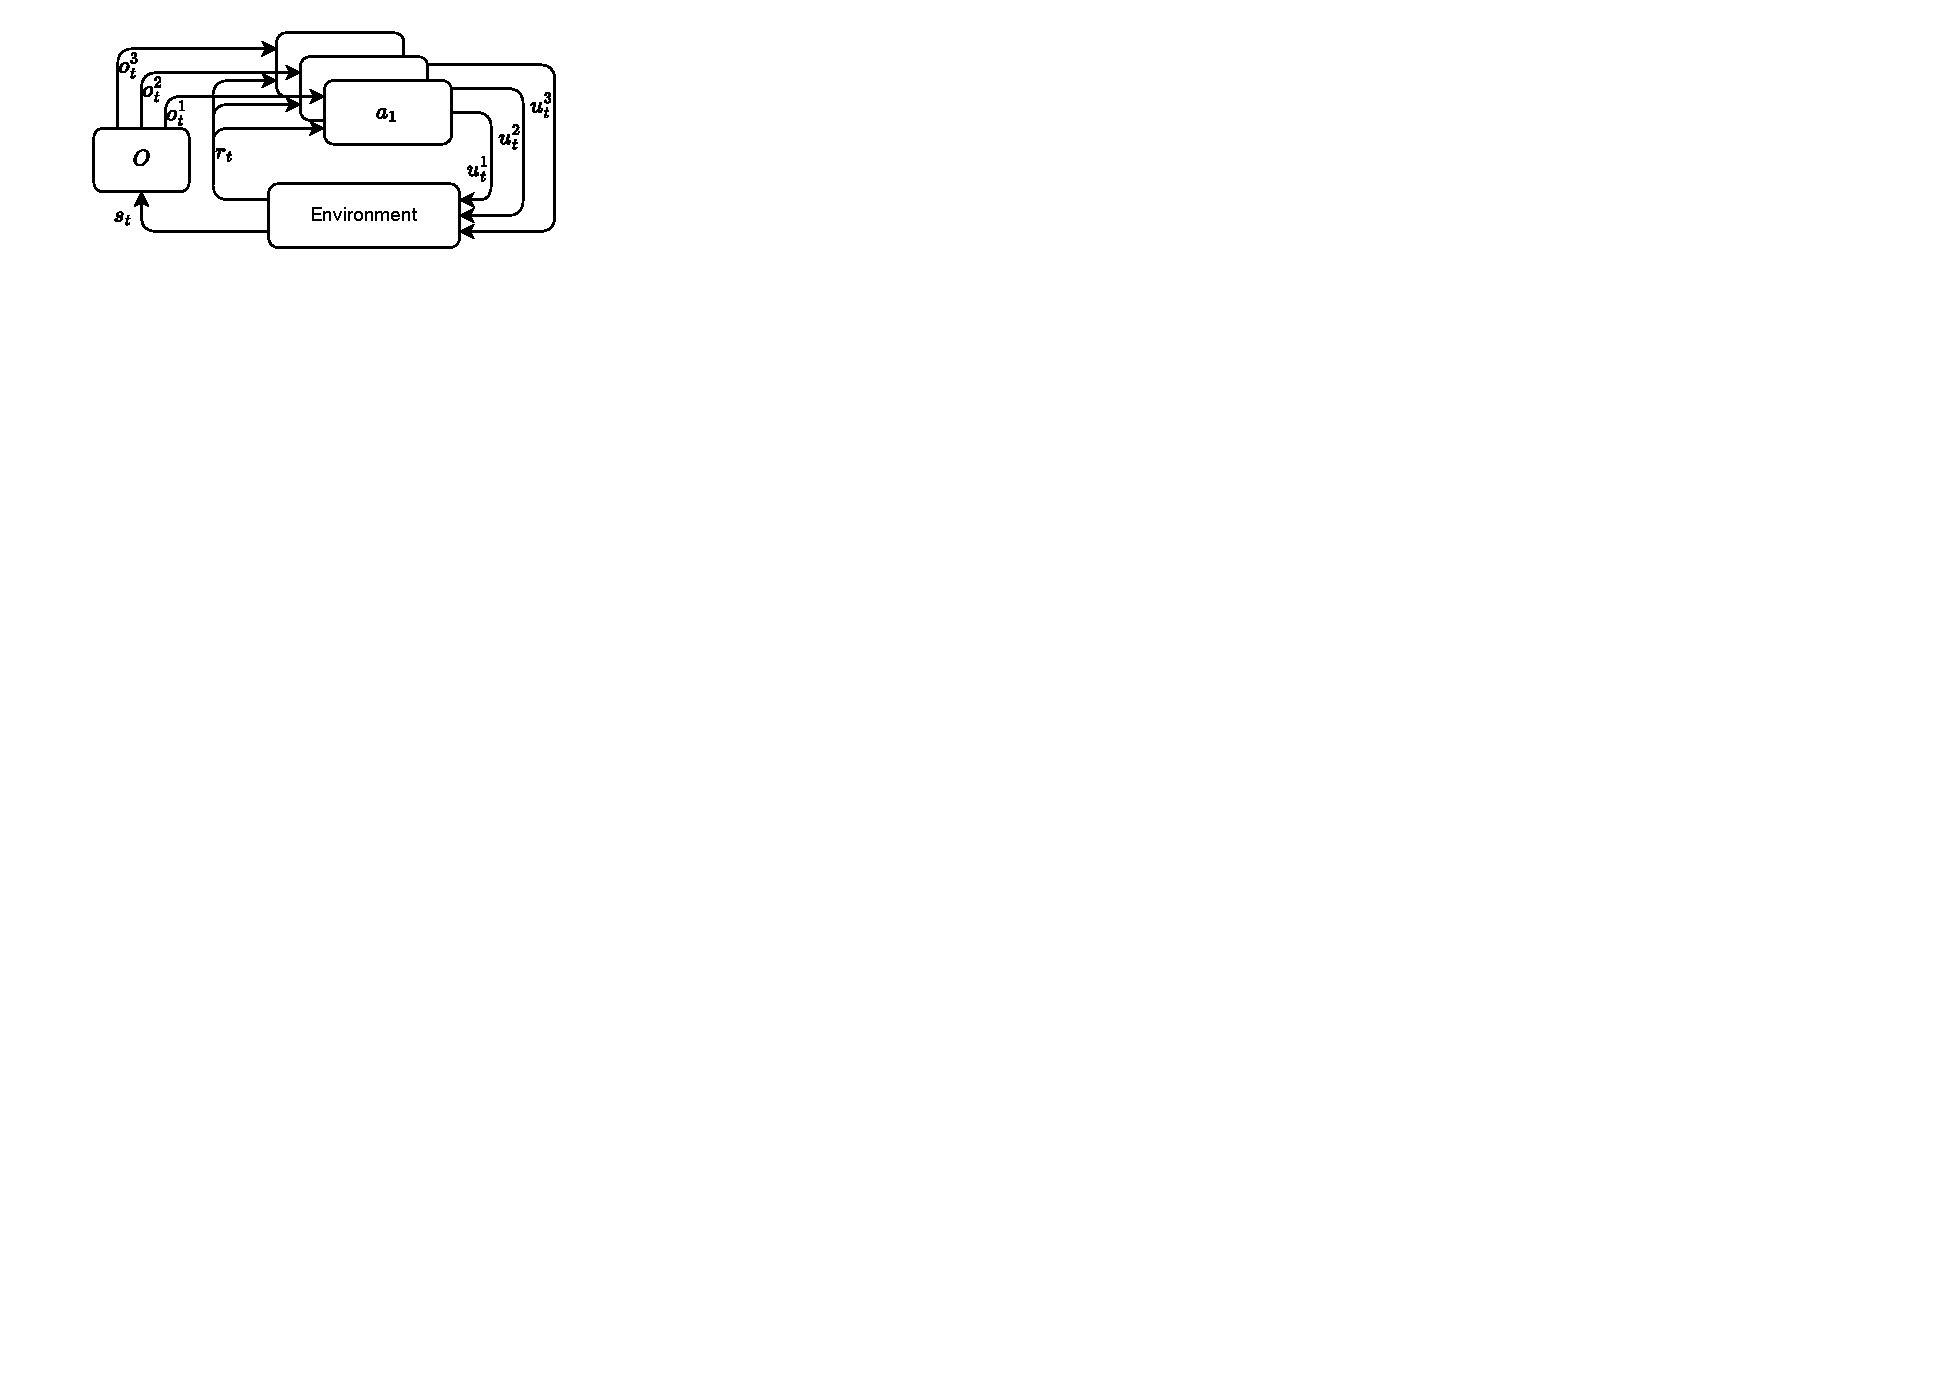
\includegraphics[width=0.8\linewidth]{tex_thesis/figures/ch3/decpomdp.pdf}
    \caption{Interaction of three agents with the environment in a decentralised partially observable Markov decision process~\citep{DecPomdp}.}
    \label{fig:ch3_decpomdp}
\end{figure}

We introduced the main challenges in MARL and will discuss hereafter the main impact of providing a common reward, which is to increase the complexity of the credit assignment problem.
Indeed, this can be considered the most complex case because all agents receive the same feedback on their actions.
The non-stationarity of learning agents and their number remains a problem.
However, choosing between two equilibria has become a trivial problem because one agent will never be disadvantaged compared to others.
Nevertheless, the common reward is not the single assumption already discussed.
Indeed, the centralised training mode also helps alleviate the complexity of these challenges.
In contrast, the decentralised mode does not consider additional assumptions besides the common reward.
The introduction may already provide some insights about this claim, and the following sections will demonstrate it.

Like MDP is the fully observable POMDP, there exist several particular cases of Dec-POMDP based on the observability of the agents.
This allows us to define the required assumptions to train a single agent to decide the joint action to make the centralised execution mode possible.
When the joint observation can identify the state while the observation of one agent can not, this is a jointly observable Dec-POMDP, also referred to as a decentralised MDP by~\cite{DecPomdp}.
However, to allow centralised execution, it should be considered that agents can share their observations to make the decision centrally by identifying the state with the joint observation.
Note that such an assumption allows centralised execution but does not make the problem of decentralised execution simpler because each agent still does not observe the state~\citep{bernstein2002complexity}.
The direct extreme case is the fully observable Dec-POMDP, where all agents observe the state directly.
These assumptions can lead to the specific framework called a multi-agent Markov decision process~\citep{boutilier1996planning}.

There are also several variations of factored Dec-POMDP described in~\citep{DecPomdp} whether the transition, reward, or observation functions can be considered factored, meaning they can be decomposed in agent-wise independent factors.
While other particular cases can be found in~\citep{DecPomdp}, their definitions allow to solve them by benefiting from additional hypotheses.
For example, in a completely factored Dec-POMDP, the decentralised mode allows to find the optimal policy, while in complex Dec-POMDP, without such a strong hypothesis, this is not always the case.
In the following, we consider CTDE algorithms that tackle the general case of Dec-POMDP, but they may have some foundation in these particular cases.

Highlighted in Section \ref{sec:ch2_partial_observability}, it is not possible to compute a belief of the state as a function of the agent's history in a Dec-POMDP because agents only access their observations and actions.
Not being able to compute a Markovian statistic induces the complexity of solving Dec-POMDP to become challenging, even more than POMDP~\citep{DecPomdp}.
For example, this forces planning methods to consider policies that map histories to action, unlike belief to action in POMDP and RL approaches defined later based on RNN, like in POMDP.
This leads the method of enumerating and evaluating all possible deterministic joint policies to select the best to be only possible for small problems.
This is because the number of possible histories grows with the length of episodes, so the number of policies to learn grows doubly exponentially with this length.

Finally,~\cite{DecPomdp} present methods that find optimal deterministic joint policy since at least one exists in finite time horizon Dec-POMDP~\citep{oliehoek2008optimal}.
These methods include dynamic programming, which solves the problem iteratively backwards, starting from the last time step of the finite horizon, pruning computed policies along the way to reduce the large number of unnecessary ones.
They also include multi-agent A*, taking foundation in search methods~\citep{russel2010} described in Chapter \ref{ch:competition}.
In short, it is a search in the space of joint policy that uses value functions as heuristics to explore the tree of possible joint policies.
\cite{DecPomdp} also present methods that do not guarantee optimality but allow to scale to a larger time horizon for the finite horizon while presenting challenges and corresponding methods to the infinite one.
Aside from the scalability issues, these methods rely on the model of the environment, motivating the use of model-free RL methods presented later in this chapter.

\section{Environments}
\label{sec:ch3_env}
Before discussing CTDE methods in detail, we provide an overview of the existing suites\footnotemark of environments in the literature.
We then describe the StarCraft multi-agent challenge (SMAC), perhaps one of the most studied environment suites in the community, but also used in our experiments in Chapter~\ref{ch:qvmix}.
Moreover, Chapter~\ref{ch:impmarl} is dedicated to a specific suite of environments, and we leave its description there.

\footnotetext{In this manuscript, an environment refers to an instance of a particular framework (here, of a Dec-POMDP). We commonly see it in the literature as either a collection of environments or an instance of one. We use "suite" to distinguish between these two.}

The multi-agent particle environments (MPE)~\citep{lowe2017multi} is a popular suite in the MARL community with cooperative scenarios.
In MPE, particles move in a 2D grid with continuous action and state spaces.
This suite comes with all types of multi-agent settings: competition, cooperation, with and without competition.
A second environment with continual action space is MaMuJoCo~\citep{peng2021facmac}.
MuJoCo~\citep{todorov2012mujoco} stands for multi-joint dynamics with contact.
It is a famous physics-based simulator to learn to control, for example, a humanoid to run.
MaMuJoCo essentially factorises MuJoCo's decisions by decentralising the decision, typically having a different agent for each leg.
It is an example of a SARL environment extended to MARL.
Other cooperative environments based on game simulators include the Hanabi Challenge~\citep{Bard_2020}, a "cooperative solitaire" between two and five players, and Google Research Football~\citep{kurach2020google}, a football game simulator.

Cooperative MARL methods are primarily benchmarked on these games and simulators, but real-world applications also exist.
City flow~\citep{zhang2019cityflow} are traffic control environments where agents control traffic lights in a city.
In Flatland~\citep{mohanty2020flatland}, agents control trains to solve a scheduling problem, avoiding collisions by coordinating trains not to take the same routes.
The multi-robot warehouse~\citep{papoudakis2021benchmarking, christianos2020shared} simulates warehouse agents needing to deliver requested goods.
Multi-Agent Tracking Environment (MATE)~\citep{NEURIPS2022_b2a1c152} is a target coverage control problem where cameras are controlled to detect all targets.
A mixed cooperative-competitive game can be made by controlling the targets.
Many more examples of cooperative MARL applications exist.
Many can be found in the books of~\cite{DecPomdp} and~\cite{marl-book}, in the review on cooperative MARL done by~\cite{oroojlooy2022review}, such as resource allocation, stock market,...


\subsection{StarCraft multi-agent challenge} \label{sec:ch3_smac}
The StarCraft multi-agent challenge (SMAC)~\citep{samvelyan2019starcraft} and its improved version SMACv2~\citep{ellis2023smacv2} are probably the most studied suite of environments with CTDE methods.
SMAC is based on the StarCraft II Learning Environment~\citep{vinyals2017starcraft}, an RL environment to play StarCraft II (SC2).
StarCraft is a strategy video game in which players compete by managing units, gathering resources, building an army, and defeating opponents.
In such games, micro-management refers to unit management, unlike macro-management, which involves resource management.
Unlike playing the real game of StraCraft like in AlphaStar~\citep{vinyals2019grandmaster}, SMAC is a suite of micro-management challenges where an independent agent controls each game unit.
Many scenarios exist in SMAC, also called "maps", and all involve training a team to achieve a common goal.
It is to defeat an adversarial team controlled by the game's deterministic and stationary policy built-in AI.
Figure~\ref{fig:ch3_smac} shows the initial configurations of two maps where two teams face each other.
Also note that in Chapter~\ref{ch:2teams}, we present a contribution where SMAC has been modified to train both competing teams.

\begin{figure}
     \centering
     \begin{subfigure}[b]{0.5\textwidth}
         \centering
         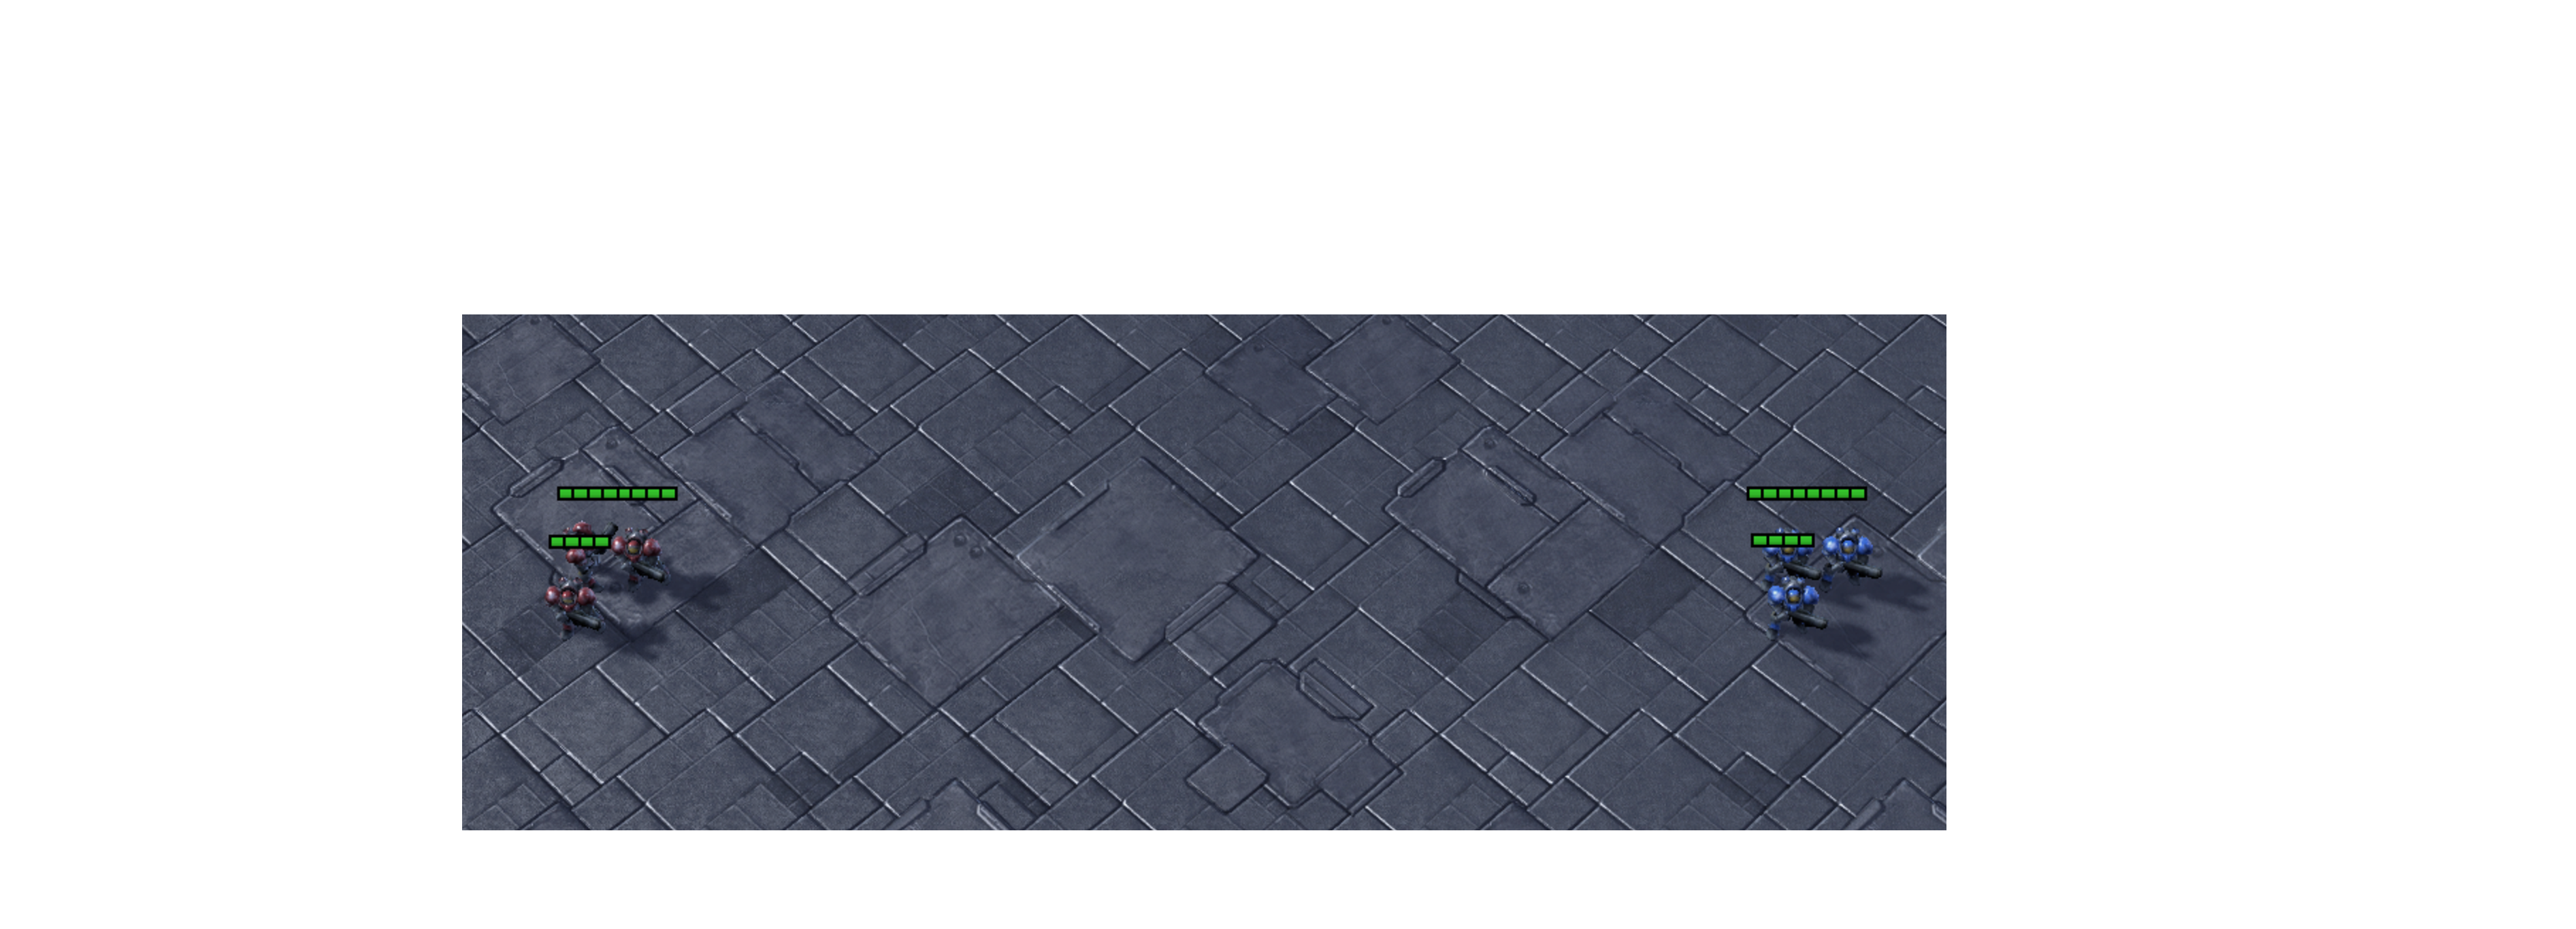
\includegraphics[height=2.3cm]{tex_thesis/figures/ch3/3m_screen.pdf}
         \caption{3m}
         \label{fig:ch3_3m}
     \end{subfigure}%
     \begin{subfigure}[b]{0.5\textwidth}
         \centering
         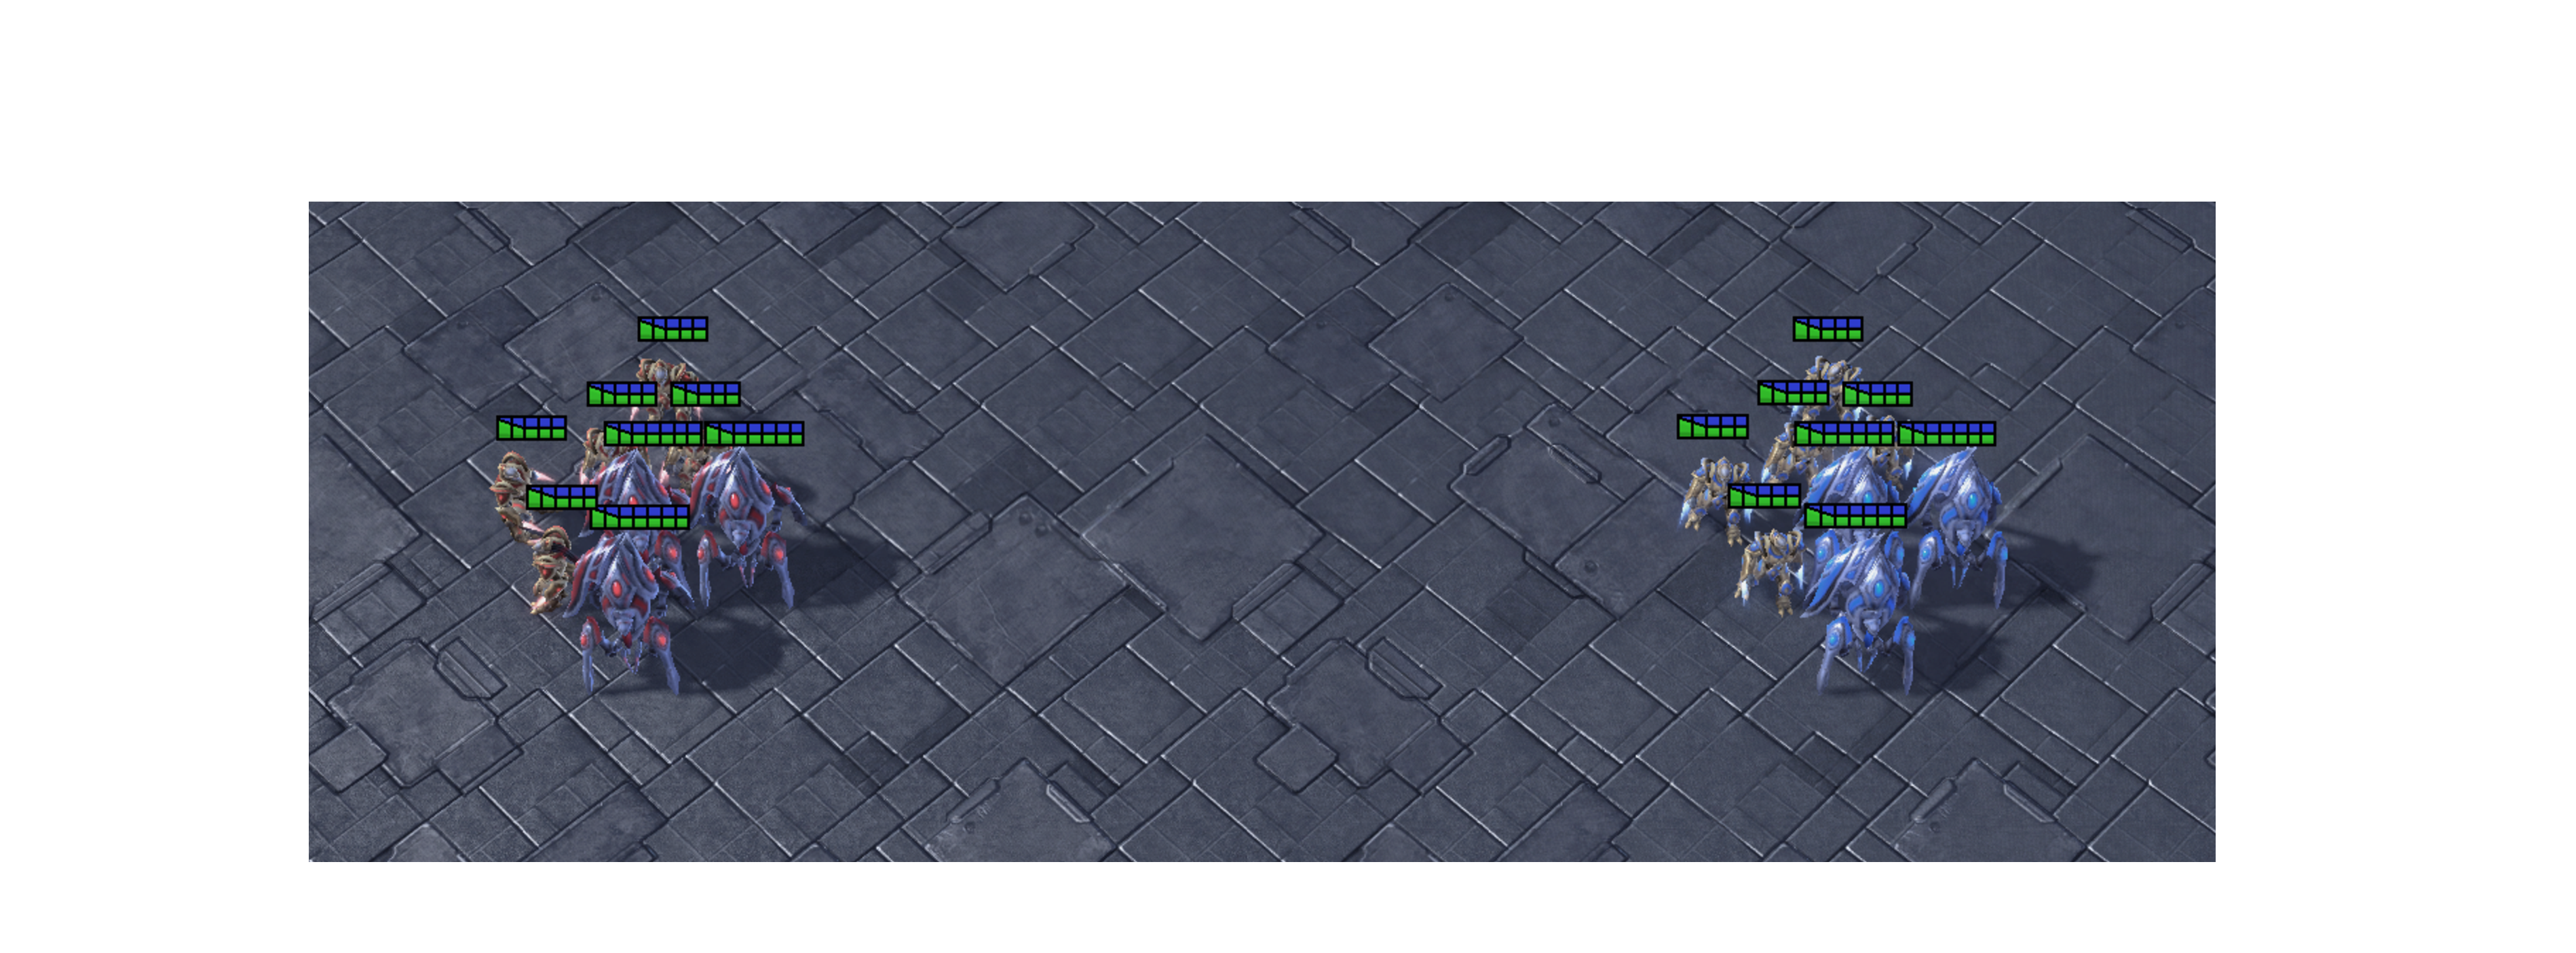
\includegraphics[height=2.3cm]{tex_thesis/figures/ch3/3s5z_screen.pdf}
         \caption{3s5z}
         \label{fig:ch3_3s5z}
     \end{subfigure}
    \caption{Two scenarios of the StarCraft multi-agent challenges.}
    \label{fig:ch3_smac}
\end{figure}

Hereafter, we thoroughly define the elements of the Dec-POMDP implemented in SMAC.
Agents have partial observability, characterised by a sight range, a circle inside which they can observe other agents.
An agent observes information about itself: its remaining hit points and shield points and four booleans representing the direction it can move in (NSWE). 
It also observes information about other agents within its sight range: the relative distance, relative x, relative y and the remaining hit points and shield points. 
If the other agent is an ally, it also observes its last performed action performed.
When the other agent is an enemy, it observes if this agent is within shooting range.
The shooting range is smaller than the sight range and depends on the unit type, and some units even attack in melee.

The state of the environment accumulates all information from agents' observations.
As described, an agent perceives other agents with distances relative to itself and does not know where it is on the map.
In the state, the agents' positions are encoded with their coordinates relative to the centre of the map.

Within all scenarios, the agent has the choice of eight actions: do nothing, move in one of four directions (NSWE) or attack one of its three opponents.
Some actions are forbidden in SMAC, such as an attack if the opponent is not within shooting range.
Therefore, agents must consider which ones are available before choosing an action.

At each time step, agents receive the same zero or positive reward. 
This reward is a sum of three factors: a zero or positive reward for the damage dealt, a positive reward if an enemy unit's hit points reach zero, and a positive reward if all enemy units are defeated. Maximisingg the reward forces the team toneutralisee every unit of the opposing team. Neutralising every opponent unit is commonly called a win in SMAC experiments.

We hereafter describe both scenarios of Figure~\ref{fig:ch3_smac}.
There are other types of units in different scenarios, and we refer the reader to~\citep{samvelyan2019starcraft}.
In the $3m$ scenario, represented in Figure~\ref{fig:ch3_3m}, six marines compete in two teams of three.
A marine has $45$ hit points and shoots at range, inflicting $6$ damage points to an opponent for each attack.
In the $3s5z$ scenario, represented in Figure~\ref{fig:ch3_3s5z}, six stalkers and ten zealots compete in two teams of eight.
Both units have shield points in addition to hit points.
A shield receives a different amount of damage and regenerates over time if the unit is not attacked again for a given time.
A stalker has $80$ hit points and $80$ shield points.
It shoots at range, inflicting $13$ damage points to the shield, $12$ damage points to a zealot's hit points and $17$ to a stalker's hit points.
A zealot has 100 hits points and 50 shield points.
It attacks in melee and inflicts $16$ damage points to the shield and $14$ damage points to the hit points of a zealot or a stalker.
All maps are presented in a video from the author\footnote{\url{https://youtu.be/VZ7zmQ_obZ0}}.

Finally, it can be intriguing to see an environment where two teams compete is considered cooperative.
This is because the built-in AI is stationary. 
These agents are not learning agents and can be considered part of the environment.
The built-in AI strategy is a rule-based policy.
Precisely, each agent moves toward the starting point of the opponent's team until it reaches the opposite side of the map and stops.
If they encounter opponents in their sight range, they select one as their target based on a priority score.
They will choose to attack the closest unit with the highest priority, which will remain the target until its priority drops or until it can no longer be attacked.
A unit's priority score is based on its type and current action.
For example, if two of the same units attack and the targeted unit stops attacking, its priority score will drop, and the built-in AI agents will select the other unit to attack.
One of the weaknesses of this built-in AI strategy that the learning agents need to learn is to stop attacking to stay alive, with the condition that an ally should be attacking.
Agents must cooperate to attack and share the possible damage inflicted by the opponents.
The following sections cover the MARL methods to achieve this coordination.

\section{Value-based methods}
\label{sec:ch3_value}

As detailed in Chapter \ref{ch:background}, value-based methods aim to learn the optimal state-action value function $Q^{\pi^*}(s, u)$, such that the optimal policy is $\pi^*(s)=\argmax_{u} Q^{\pi^*}(s, u)$.
In SARL, one solution, called DQN, is to approximate $Q$ with a neural network $\theta$ and learn $Q(s, u;\theta)$
by minimising the loss defined in Equation~\ref{eq:ch2_dqnloss}.
We hereafter describe how to train agents with value-based methods and the different modes of training and execution.

As introduced in Section~\ref{sec:ch3_intro}, there exist different modes of training and execution.
In the first mode, one possible centralised training and execution approach is to train a centralised learner with DQN in a Dec-POMDP.
Remind that it is only possible if the Dec-POMDP is a multi-agent Markov decision process~\citep{boutilier1996planning}.
In this setting, the centralised agent learns the state-joint-action value function $Q^{\mathbf{\pi}}(s,\mathbf{u}; \theta)$ by following the adapted DQN loss
\begin{equation}
\label{eq:ch3_centralQloss}
    \mathcal{L}(\theta) = \mathbb{E}_{B} \big[\big(r_{t} + \gamma \max_{\mathbf{u}} Q(s_{t+1}, \mathbf{u}; \theta')- Q(s_{t}, \mathbf{\mathbf{u_t}}; \theta)\big)^{2}\big].
\end{equation}
Issues are that the joint action space scales exponentially with $n$.
Also, in practice, agents select their action based only on their history $(o, \tau)$ and not the state $s$.

For the second mode, the decentralised training and execution, each agent can learn its own Q-value independently $Q_a=Q(\tau^a, u^a)$, agnostically of the existence of other agents.
IQL~\citep{Tan1993} is the extension of Q-Learning (see Chapter~\ref{ch:background}) to this mode. 
The equivalent extension has been performed with DQN~\citep{TampuuDqnIQL}, also called IQL.
Typically, in a Dec-POMDP, a recurrent network approximates the independent Q-value, as explained in Section \ref{sec:ch2_partial_observability}.
One problem with IQL is that agents must select actions which maximise $Q(s_t, \mathbf{u_t})$ while ignoring, at any time, actions taken by other agents.

This is where centralised training with decentralised execution (CTDE), the third mode, comes in handy.
The objective is to ensure that actions $\mathbf{u_t}$ maximising the individual $Q_a(\tau_t^a, u_t^a))$ functions also maximise $Q(s_t, \mathbf{u_t})$.
With CTDE methods, this is made possible by approximating this $Q(s_t, \mathbf{u_t})$ as a factorisation of individual $Q_a$ functions during training.
To ensure this, individual $Q_a$ functions must satisfy the individual-global-max condition (IGM)~\citep{Son2019QTRAN:Learning}
\begin{equation}
    \argmax_{\mathbf{u_t}} Q(s_t, \mathbf{u_t}) =(\argmax_{u_t^{1}} Q_{1}(\tau_t^{1}, u_t^{1}),...,\argmax_{u_t^{n}} Q_{n}(\tau_t^{n}, u_t^{n})).
    \label{eq:ch3_igm}
\end{equation}

Satisfying the IGM property allows agents to greedily select actions that maximise their individual $Q_a$ and the state-joint-action value function $Q(s_t, \mathbf{u_t})$.
Therefore, during training, an approximation of $Q(s_t, \mathbf{u_t})$, sometimes denoted $Q_{tot}$, is built as a factorisation of $Q_a$ and then dropped at execution.
Agents select actions based on these $Q_a$, satisfying IGM, and only these networks are kept for the execution.
Note that these $Q_a$ are now utility functions because they do not approximate the expected sum of discounted rewards.
In this manuscript, we express $Q_{tot}$ as a function of the state $s$ and consider that the state is known.
However, it can be rewritten as a function of the joint history $\mathbf{\tau}$ if the state $s$ is unknown during training.

Maybe one of the first CTDE methods of value-based factorisation is called value decomposition network (VDN)~\citep{sunehag2018vdn}.
This method factories $Q_{tot}$ using the addition, an operation which satisfies IGM: $Q_{tot}^{VDN}(s_t, \mathbf{u_t}) = \sum_{i=1}^n Q_{a_i}(\tau^{a_i}_t, u^{a_i}_t)$.
One limitation of VDN, leaving the details of the training procedure for later, is that factorising through addition does not allow the creation of a complex approximation of the joint-action-state Q functions.
Another limitation is that $Q_{tot}$ is needed only during training, and in VDN, it does not benefit from additional information, such as the state.
In the following, we present three methods for improving VDN.
These three have been tested in the contributions presented in later chapters.
Other methods exist, and we finish this section with a related work discussion.

\subsection{QMIX}
QMIX~\citep{Rashid2018} is a CTDE method where the approximation of $Q_{tot}$ is performed by a monotonefactorisationn of the individual $Q_a$ functions while also being a function of the state:
\begin{equation}
     Q_{tot}^{mix}(s_t, \mathbf{u_t})=\text{Mixer} \left(Q_{a_1}(\tau^{a_1}_t, u_t^{a_1}) ,..,Q_{a_n}(\tau^{a_n}_t, u_t^{a_n}), s_t\right).
     \label{eq:ch3_qmixappendix}
\end{equation}

The monotonicity is ensured by a hypernetwork~\citep{Ha2016HyperNetworks} $h_p(.): \mathcal{S} \rightarrow \mathbb{R}^{|\phi|+}$ which computes, from the state $s_t$, the parameters $\phi$ of a mixer network $h_m(.;\phi):\mathbb{R}^n \times \phi \rightarrow \mathbb{R}$.
To ensure monotonicity, the weights (and not the biases) defined by $\phi$ are constrained to be positive.
Together, $h_p$ and $h_m$ defines the mixer such that $ Q_{tot}^{mix}(s_t, \mathbf{u_t}) = h_m\left(Q_{a_1},..,Q_{a_n}; h_p(s_t)\right)$.

The monotonicity of $Q_{tot}^{mix}$ with respect to the individual $Q_a$ functions, 
\begin{equation}
    \frac{\partial Q_{tot}^{mix}(s_t, \mathbf{u_t})}{\partial Q_{a}(s_t, u_t^{a})} \geq 0 \text{ } \forall a
    \label{eq:ch3_monotonicity},
\end{equation}
is satisfied because a neural network comprised of monotonic functions ($h_m$) and strictly positive weights ($h_p$) is monotonic with respect to its inputs ($Q_a$). 
The entire QMIX architecture is presented in Figure~\ref{fig:qmix}.

\begin{figure}
\centering

\begin{tikzpicture}[node distance=.5cm]

\tikzstyle{netbox} = [rectangle, rounded corners, minimum width=1cm, minimum height=1cm, draw=blue]
\tikzstyle{mixerbox} = [rectangle, rounded corners, minimum width=4.5cm, minimum height=1.5cm, draw=blue]
\tikzstyle{indixQbox} = [rectangle, rounded corners, minimum width=1.3cm, minimum height=2cm, draw=red, line width=1pt]
\tikzstyle{io} = [minimum width=0.2cm,minimum height=0.5cm]
\tikzstyle{emptynetbox} = [rectangle, rounded corners, minimum width=1cm, minimum height=1cm]

\node (output_node) [io] {$Q_{mix}^{tot}(s_t, \mathbf{u_t})$};
\node (mixerbox) [mixerbox, below=of output_node, yshift=-0cm, label={[xshift=-1.4cm, yshift=-1cm]Mixer}] {};
\node (indivQbox1) [indixQbox, below=of mixerbox, xshift=-1.2cm, yshift=-.5cm, label={[xshift=-0.22cm, yshift=.2cm]$Q_{a_1}(\tau^1_t, u^1_t)$}] {$Q_{a_1}$};
\node (indivQboxn) [indixQbox, below=of mixerbox, xshift=1.2cm, yshift=-.5cm, label={[xshift=0.22cm, yshift=.2cm]$Q_{a_n}(\tau^n_t, u^n_t)$}] {$Q_{a_n}$};
\node (mixer_net) [netbox, below=of output_node, yshift=-0.3cm] {$h_m$};
\node (param_net) [netbox, right=of mixer_net] {$h_p$};
\node (param_net2) [emptynetbox, left=of mixer_net] {};


\node (intput_node1) [io,below=of indivQbox1, yshift=-0cm, label={[xshift=1.2cm, yshift=1.2cm]. . .}] {$o^{a_1}_t$};
\node (intput_noden) [io,below=of indivQboxn, yshift=-0cm] {$o^{a_n}_t$};
\node (intput_nodestate) [io, right=of param_net] {$s_t$};
\node (intput_nodestate2) [io, left=of param_net2] {};

\draw [-Latex, thick] (intput_node1) -- (indivQbox1);
\draw [-Latex, thick] (intput_noden) -- (indivQboxn);
\draw [-Latex, thick] (indivQbox1) --  (mixer_net);
\draw [-Latex, thick] (indivQboxn) -- (mixer_net);
\draw [-Latex, thick] (param_net) -- (mixer_net) node[midway, yshift=0.3cm] {$|.|$};
\draw [-Latex, thick] (intput_nodestate) -- (param_net);
\draw [-Latex, thick] (mixer_net) -- (output_node);

%\draw[thick, rounded corners, draw=blue, fill=blue!50, opacity=0.2] ($(mixerbox.north west)+(-0.5,0.5)$) rectangle ($(indivQboxn.south east)+(1,-0.5)$);
\draw[thick, rounded corners, fill=red!50, opacity=0.2] ($(indivQbox1.north west)$) rectangle ($(indivQbox1.south east)$);
\draw[thick, rounded corners, fill=red!50, opacity=0.2] ($(indivQboxn.north west)$) rectangle ($(indivQboxn.south east)$);
\end{tikzpicture}
\caption{QMIX architecture.}
\label{fig:qmix}
\end{figure}

The optimisation procedure follows the same principles of the DQN algorithm, and the loss applied to $Q_{mix}(s_t, \mathbf{u_t})$ is 
\begin{equation}
    \mathcal{L}(\theta) = \mathbb{E}_{B}
    \bigg[  
    \big(r_{t} + \gamma \max_{\mathbf{u} \in \mathcal{U}} Q_{tot}^{mix}(s_{t+1}, \mathbf{u}; \theta')
    - Q_{tot}^{mix}(s_{t}, \mathbf{u_{t}}; \theta)\big)^{2}
    \bigg].
    \label{eq:QMIX_loss}
\end{equation}
During training, actions are selected with an epsilon greedy policy from $Q_a$.
At testing, actions are selected with a greedy policy.
Individual $Q_a$ networks and the mixer are all copied to produce target networks represented by $\theta'$.

\begin{figure}
    \centering
\begin{tikzpicture}[node distance=.5cm]

\tikzstyle{netbox} = [rectangle, rounded corners, minimum width=2cm, minimum height=0.5cm,text centered, draw=red]
\tikzstyle{io} = [minimum width=0.2cm,minimum height=0.5cm, text centered]

\node (output_node) [io] {$\{Q_a(o_t^a, u^a_{j}) \forall u^a_j \in \mathcal{U}_a \}$};
\node (fctop) [netbox, below=of output_node, yshift=-0.3cm] {FC layer};
\node (rec_net) [netbox, below=of fctop, text width=2cm] {Recurrent layer};
\node (fcbot) [netbox, below=of rec_net] {FC layer};
\node (input_node) [io,below=of fcbot, yshift=-0.3cm] {$o^a_t$}%, u^a_{t-1}$};
\node (input_rec) [io,left=of rec_net, xshift=-0.3cm] {$h_{t-1}$};
\node (output_rec) [io,right=of rec_net, xshift=+0.3cm] {$h_t$};

\draw [-Latex, thick] (input_node) -- (fcbot);
\draw [-Latex, thick] (fcbot) -- (rec_net);
\draw [-Latex, thick] (rec_net) -- (fctop);
\draw [-Latex, thick] (fctop) -- (output_node);
\draw [-Latex, thick] (input_rec) -- (rec_net);
\draw [-Latex, thick] (rec_net) -- (output_rec);

\draw[thick, rounded corners, draw=red, fill=red!50, opacity=0.2] ($(fctop.north west)+(-0.5,0.5)$) rectangle ($(fcbot.south east)+(0.5,-0.5)$);
\draw[thick, rounded corners, draw=red] ($(fctop.north west)+(-0.5,0.5)$) rectangle ($(fcbot.south east)+(0.5,-0.5)$);
\end{tikzpicture}
\caption{Common $Q_a$ network implementation. The hidden state $h$ embeds the history, and the action space size defines the number of outputs of the network.}
\label{fig:ch3_indivQ}
\end{figure}

Since the Dec-POMDP induces partial observability, individual $Q_a$ networks are commonly RNNs made of GRU~\citep{Chung2014EmpiricalModeling} and the replay buffer stores sequences of contiguous transitions instead of isolated transitions $\langle s_{t},\mathbf{u_{t}},r_{t},s_{t+1}\rangle$.
A typical architecture of such a network is presented in Figure \ref{fig:ch3_indivQ}.
When evaluating CTDE methods, IQL is commonly tested by training the same architecture as the individual network, allowing for comparison with a fully decentralised training of such a network.

\subsection{MAVEN}
\citet{Mahajan2019MAVEN:Exploration} defined the class of state-joint-action value functions that QMIX cannot represent due to its exploration strategy and the monotonicity constraint.
They demonstrated the existence of payoff matrices in an n-player normal-form game with more than three actions per agent, for which QMIX learns a suboptimal policy for any training duration, using both epsilon greedy and uniform exploration.
To tackle this problem, they modified the individual $Q_a$ architecture, which is now a function of the latent space to influence agent behaviour.
The underlying objective is to train agents to learn an ensemble of policies to improve their exploration capabilities.

Specifically, the latent variable is the input of a second and new hypernetwork that computes parameters of the fully connected layer linking recurrent cells to the outputs of the individual $Q_a$ networks.
This latent variable $z$ is generated per episode by a hierarchical policy network, taking as input the initial state of the environment and a random variable (typically a discrete uniform).
The idea is that the latent variable corresponds to different learnt strategies.
The goal of the hierarchical policy network is to select the best strategy based on the initial state $s_0$, which is considered known at testing.
The new architecture of the individual $Q_a$ network of MAVEN is represented in Figure~\ref{fig:maven}.

\begin{figure}
\centering
\begin{tikzpicture}[node distance=.5cm]

\tikzstyle{netbox} = [rectangle, rounded corners, minimum width=1.6cm, minimum height=0.7cm,text centered, draw=red]
\tikzstyle{netboxMaven} = [rectangle, rounded corners, minimum width=2cm, minimum height=0.7cm,text centered, draw=green]
\tikzstyle{io} = [text centered]

\node (output_node) [io] {$\{Q_a(s_t, u^a_{j}) \forall u^a_j \in \mathcal{U}_a \}$};
\node (fctop) [netbox, below=of output_node, yshift=-0.3cm] {FC layer};
\node (rec_net) [netbox, below=of fctop, text width=2cm] {Recurrent layer};
\node (fcbot) [netbox, below=of rec_net] {FC layer};
\node (intput_node) [io,below=of fcbot, yshift=-0cm] {$o^a_t, u^a_{t-1}$};
\node (input_rec) [io,left=of rec_net, xshift=-0.1cm] {$h_{t-1}$};
\node (output_rec) [io,right=of rec_net, xshift=+0.05cm] {$h_t$};

\draw [-Latex, thick] (intput_node) -- (fcbot);
\draw [-Latex, thick] (fcbot) -- (rec_net);
\draw [-Latex, thick] (rec_net) -- (fctop);
\draw [-Latex, thick] (fctop) -- (output_node);
\draw [-Latex, thick] (input_rec) -- (rec_net);
\draw [-Latex, thick] (rec_net) -- (output_rec);



\node (param_net) [netboxMaven, right=of fctop, xshift=1cm, text width=2.45cm] {Hypernetwork};
\node (latentvar) [io, right=of rec_net, xshift=.66cm, text width=2.5cm] {$z$};
\node (latent_net) [netboxMaven, right=of fcbot, xshift=1cm, text width=2.5cm] {Hierarchical policy network};
\node (intput_latent_1) [io,below=of latent_net, yshift=-0cm, xshift=-0.8cm] {$s_{t_0}$};
\node (intput_latent_2) [io,below=of latent_net, yshift=-0cm, xshift=0.8cm] {$x \sim P(x)$};
\draw [-Latex, thick] (param_net) -- (fctop);
\draw [-Latex, thick] (latentvar) -- (param_net);
\draw [-Latex, thick] (latent_net) -- (latentvar);
\draw [-Latex, thick] (intput_latent_1) -- (latent_net);
\draw [-Latex, thick] (intput_latent_2) -- (latent_net);


\draw[thick, rounded corners, draw=red, fill=red!50, opacity=0.2] ($(fctop.north)+(-1.5,0.3)$) rectangle ($(fcbot.south)+(1.5,-0.3)$);
%\draw[thick, rounded corners, draw=green, fill=green!80, opacity=0.2] ($(param_net.north)+(-1.5,0.3)$) rectangle ($(latent_net.south)+(1.5,-0.3)$);
\draw[thick, rounded corners, draw=red] ($(fctop.north)+(-1.5,0.3)$) rectangle ($(fcbot.south)+(1.5,-0.3)$);
\draw[thick, rounded corners, draw=green] ($(param_net.north)+(-1.5,0.3)$) rectangle ($(latent_net.south)+(1.5,-0.3)$);


\end{tikzpicture}
\caption{MAVEN modification of the individual $Q_a$ network.}
\label{fig:maven}
\end{figure}

MAVEN's network objective function comprises three parts.
Some parameters must be fixed when computing some parts, meaning all parameters are not updated based on all objectives.
The first part of the objective is the loss of QMIX defined in Equation~\ref{eq:QMIX_loss}, and it optimises both hypernetworks and individual networks.
This loss is computed by fixing the hierarchical policy network and, thus, the latent variable $z$.

The hierarchical policy network can be optimised with any policy-based method, such as policy gradient maximising the sum of rewards per episode, defined in Section \ref{sec:ch2_policy_based_methods}.
This second objective is computed by fixing both hypernetworks and individual networks.

The third part of the objective ensures that different values of $z$ imply different behaviours. 
It is a mutual information loss between the latent variable and the trajectories performed by agents to favour different behaviours for different latent variable values.
For further details on the MAVENoptimisationn procedure and especially on constructing the mutual information objective, we refer the reader to~\cite{Mahajan2019MAVEN:Exploration}.

\subsection{QPLEX}
QPLEX~\citep{wang2021qplex} extends QMIX with the dueling structure $Q(s_t, u_t) = V(s_t) + A(s_t, u_t)$~\citep{wang2016dueling}, learning a factorisation of $V$ and $A$ with transformers~\citep{vaswani2017attention}.
The advantage function $A$ has been introduced in Section \ref{sec:ch2_policy_based_methods}.
The duelling structure involves learning $V(s_t)$ and $A(s_t, u_t)$, typically with a single neural network with a common backbone and two different heads.
By separating the computation of the value of a given state and the contributions of different actions in that given state,~\citet{wang2016dueling} demonstrated better results than DQN.

Back to QPLEX,~\citet{wang2021qplex} demonstrated that if the advantage function $A$ respects the advantage-IGM, then the state action value function $Q = V + A$ respect IGM while removing constraints on the state value function $V$.
The individual $Q_a$ satisfy the advantage-IGM if $Q_{tot}=V_{tot}+A_{tot}$ and $V_{tot}(s)=\max_{\mathbf{u}} Q_{tot}(s, \mathbf{u})$ and $Q_a=V_a+A_a$ and $V_a(s)=\max_{u} Q_a(s, u)$ such that 
\begin{equation}
    \argmax_{\mathbf{u_t}} A_{tot}(s_t, \mathbf{u_t}) =(\argmax_{u_t^{1}} A_{1}(\tau_t^{1}, u_t^{1}),...,\argmax_{u_t^{n}} A_{n}(\tau_t^{n}, u_t^{n}))    
\label{eq:ch3_adv_igm}
\end{equation}
holds.
This defines the duplex dueling structure of QPLEX.
The constraint on the $Q_a$ is transferred to the advantage functions $A_i$, leading to an unconstrained approximation of the state value function $V$.

\subsection{Other value-based methods}
In addition to QMIX~\citep{Rashid2018}, QVMix~\citep{leroy2020qvmix} and QPLEX~\citep{wang2021qplex}, Qatten \citep{yang2020qatten} is another example of $Q_{tot}$ factorisation with transformers.
Other, such as QTRAN~\citep{Son2019QTRAN:Learning} and Weighted-QMIX~\citep{rashid2020weighted}factorisee $Q_{tot}$ differently from the QMIX and VDN approach to improve the representational capacity of the factorisationn.
However, they end up not always satisfying IGM.
Other methods learn to cooperate without factorising $Q_{tot}$ to satisfy IGM.
An example is local advantage network (LAN)~\citep{avalos2023local}, which learns a central state value function of the joint policy $V^{\mathbf{\pi}}$ and individual advantages $A^a$ to learn $Q_a$ during training, keeping only $A_a$ at execution.
There are many other methods relying on the value function decomposition.
Finally, \cite{hong_rethinkigm} claims that many have been trying to improve the $Q_{tot}$ factorisation to satisfy IGM, but only a few examine IGM defects.
Lossy decomposition occurs when the actions that maximise $Q_{tot}$ are not the ones maximising $Q_a$.
They demonstrate the existence of lossy decomposition when the observation of one agent is characterised as insufficient.
An observation is insufficient when it does not change when the state changes. 
This claim is somehow similar to the one of \cite{Mahajan2019MAVEN:Exploration}, who demonstrated the existence of games where QMIX cannot correctly approximate  $Q_{tot}$, focusing on the reward structure.
This highlights some remaining challenges in CTDE value-based methods.

\section{Policy-based methods}
\label{sec:ch3_policy}

Agents trained with policy-based methods learn the policy with a neural network, as introduced in Chapter \ref{ch:background}, and we hereafter describe actor-critic methods adapted to the Dec-POMDP.
As demonstrated with DQN in the previous section, in the centralised mode, it is possible to train an agent with a SARL solution to select actions in the joint action space.
In the decentralised mode, the equivalent to IQL for policy-based methods is named IAC~\citep{foerster2017coma}.
The policies learned by the actor of each agent is $\pi^{a}(u_t^{a}|\tau_t^{a}, o^a_t;\theta)$.
The policy parameters are updated by ascending the gradient
\begin{equation}
\label{eq:ch3_policy_grad}
    \nabla_\theta J(\pi^a_\theta) = \mathbb{E}_B\left[A_a(\tau^{a}_t, o_t^a, u_t^{a}; \phi) \nabla_{\theta} \log \pi^{a}(u_t^{a}|\tau_t^{a},  o_t^a;\theta)\right].
\end{equation}
As in SARL, there are two possible ways of estimating the advantage with a critic network.
This leads to two IAC versions: IAC-V where a state value function is learned $A_a(\tau_t, u_t; \phi) = r + \gamma V_a(\tau_{t+1}; \phi) - V_a(\tau_t; \phi)$ and IAC-Q, where a state-action value function is learned $A_a(\tau_t, u_t; \phi) = Q_a(\tau_t, u_t; \phi) - \sum_{u^a}\pi_\theta(\tau_t, u^a)Q_a(\tau_t, u^a; \phi)$.
The parameters of $\pi^a$ and $Q_a$ are denoted $\theta$ or $\phi$ and not $\theta_a$ or $\phi_a$ to improve readability, although they might be shared or not by agents.

In IAC, each agent independently learns an actor and a critic, but this solution does not benefit from any additional information, such as the state $s$.
Since critics are used only during training, one straightforward solution is to exploit the state $s$ to compute a centralised critic.
Moreover, the critic is trained to update the policy network and plays a crucial role in each agent's credit assignment.
We hereafter detail two methods that consider a single centralised critic exploiting the state tested in the contributions presented in later chapters.
Other methods exist, and we finish this section with a related work discussion.

\subsection{COMA}
\label{sec:ch3_coma}

COMA stands for counterfactual multi-agent policy gradient and is a solution proposed by~\cite{foerster2017coma}.
They motivate their approach with the constatation that a centralised critic computing the advantage $A_a(s_t, u^a_t) = r_t + \gamma V(s_{t+1}; \phi) - V(s_t; \phi)$ is based on the common reward $r_t$ but does not consider how the action of an individual agent influences it.
Such a centralised critic does not solve the credit assignment problem.

\cite{foerster2017coma} propose to use a counterfactual baseline inspired by difference rewards $D_t^a=R(s_{t+1}, s_t, \mathbf{u_t}) - R(s_{t+1}, s_t, (\mathbf{u_t^{-a}}, c_t^a))$~\citep{wolpert2001optimal}.
The common reward $R(s_{t+1}, s_t, \mathbf{u_t})$ is compared to a reward obtained when agent $a$ executes a default action $c^a$, while we preserve actions of other agents $\mathbf{u_t^{-a}}$ unchanged.
Any action $u^a$ that maximises $R(s_{t+1}, s_t, \mathbf{u_t})$ also maximises $D_t^a$.
However, there are immediate limitations.
First, the simulator needs to be run to obtain this "default reward" $R(s_{t+1}, s_t, (\mathbf{u_t^{-a}}, c_t^a))$.
And this must be done for all agents.
Second, if we consider it possible to approximate it, this would induce additional approximation error.
Third, the choice of the default action is not trivial.

The COMA solution to these limitations is to build a centralised critic that computes difference rewards by learning $Q(s, \mathbf{u})$.
For each agent $a$, the advantage updating actor networks in Equation \ref{eq:ch3_policy_grad} is 
\begin{equation}
\label{eq:ch3_coma_adv}
A_a(s_t,\mathbf{u_t}; \phi)=Q(s_t, \mathbf{u_t};\phi) - \sum_{u'^{a}} \pi^a({u'^{a}} |\tau_t^a, o_t^a;\theta) Q(s_t, (\mathbf{u_t^{-a}}, u'^{a}); \phi).
\end{equation}
This solves the problems of simulating the default rewards and choosing default actions.
However, $|\mathcal{U}^1|+...+|\mathcal{U}^n|$ values must be computed to obtain the advantage of all agents.
In practice, a $Q$ network has one output for each possible action.
Here, this leads to $\sum_{i=1}^n|\mathcal{U}^i|$ outputs which would become impractical whether $n$ or $|\mathcal{U}^a|$ increases.
To alleviate this, the critic can take as input $\mathbf{u^{-a}}$ and only outputs $|\mathcal{U}^a|$ outputs.
To use the same critic for all agents implies that all action spaces are the same size.

A significant limitation is that this method is only possible for discrete action spaces, especially considering the sum over all actions in the advantage.
\cite{foerster2017coma} argue that it would be possible to apply COMA with continuous action spaces easily by evaluating $\sum_{u'^{a}} \pi^a(u'^{a}|\tau^a) Q(s,(\mathbf{u^{-a}},u'^{a}))$ with Monte-Carlo estimations or by using policy construction that allows to compute it anatically.
A final observation is that the critic is considered central because using the state $s_t$, but it should be called $n$ times to update the $n$ actor networks.

In COMA, policy networks $\theta$ usually follow the same architecture of IQL presented in Figure \ref{fig:ch3_indivQ}, where the outputs are not $Q$ values for each action but the probability of taking each action, usually obtained by applying a softmax to the last layer.
The critic is commonly composed of fully connected layers that output the $|\mathcal{U}^a|$ from the state $s_t$, the actions of others $\mathbf{u_t^{-a}}$ and sometimes additional information, such as $o_t^a$ or the previous taken action $\mathbf{u_{t-1}}$.

\subsection{FACMAC}

FACMAC~\citep{peng2021facmac} stands for factored multi-agent centralised policy gradients.
They propose to use a centralised but factored critic computing $Q_{tot}$ as a factorisation of individual $Q_a$, like in QMIX.
In COMA, the critic is centralised because it has access to the state, but all agents use it independently to update their decentralised policy.
\cite{peng2021facmac} calls this approach a monolithic critic, and they argue that a non-monolithic factored critic is preferable to scale to many agents or actions.
In addition, they show that estimating gradients independently for each agent can yield sub-optimal joint policies.
This motivates the centralised and factored critic which computes a single gradient estimate for the joint policy, improving cooperation capabilities.

Conversely to COMA, FACMAC is designed for continuous action spaces and can be adapted to discrete ones.
It is built on the same foundation of another actor-critic method for MARL developed to solve a stochastic game called multi-agent deep deterministic policy gradient (MADDPG)~\citep{lowe2017multi}.
The latter is a multi-agent version of DDPG~\citep{lillicrap2015continuous}, an actor-critic method using deep neural networks to approximate a deterministic policy and a $Q$ function in SARL.
Since the action space is continuous, obtaining the action $\argmax_u Q(s, u)$ can be difficult.
Instead of computing the arg max, the solution in DDPG is to learn a parametrised deterministic policy $\mu_\theta:\mathcal{S}\rightarrow\mathcal{U}$ that solves $\max_\theta \mathbb{E}_B[Q(s, \mu_\theta(s); \phi)]$ by gradient ascent, while the critic estimates this $Q$~\citep{silver2014deterministic}.
MADDPG uses DDPG to learn decentralised policies using centralised critics with access to the state and actions of other agents.
In MADDPG, each decentralised actor $\mu^a(\tau^a, o^a;\theta)$ is updated by ascending the gradient
\begin{equation}
\label{eq:ch3_maddpg_grad}
    \nabla_\theta J(\mu^a) = \mathbb{E}_B\left[\nabla_{\theta} \mu^a(\tau_t^a, o_t^a;\theta) \nabla_{u^a} Q_a^{\mathbf{\mu}}(s_t, \mathbf{u_t^{-a}}, u a; \phi)|u^a=\mu^a(\tau_t^a, o_t^a)\right],
\end{equation}
where actions of other agents are taken from the replay buffer while the action of agent $a$ is provided by its deterministic policy when computing the state-joint-action value function.
The critic is updated following the same centralised loss adapted from DQN defined in Equation \ref{eq:ch3_centralQloss} where, in addition to a target network to compute $Q$, actions of agents to compute this target value are taken from target deterministic policies.
While MADDPG addresses stochastic games with individual rewards, it can be applied easily in Dec-POMDP, with the drawbacks mentioned earlier.
Note that the critic of MADDPG is monolithic and different for each agent, like COMA.

Using a single centralised and factored critic is FACMAC's change to MADDPG.
All agents share this critic that computes $Q_{tot}^{\mathbf{\mu}}$ where $\mathbf{\mu}$ is the joint deterministic policy.
Like the CTDE value-based methods, $Q_{tot}$ is a function of individual utility functions $Q_a$.
The factorisation can be done by a sum, such as in VDN, or by a hypernetwork, such as in QMIX in Equation \ref{eq:ch3_qmixappendix}.
However, the monotonicity constraint to satisfy IGM is not required for a critic.

The factored critic does not replace how $Q$ is computed in Equation \ref{eq:ch3_maddpg_grad}.
Indeed, in MADDPG, actors are updated based on $\mathbf{u_t^{-a}}$ stored in the replay buffer, which can lead to sub-optimal joint policies.
Instead, FACMAC computes a single gradient based on the current joint policy $\mathbf{\mu}(\mathbf{\tau}, \mathbf{o}) = (\mu^{a_1}(\tau^{a_1}, o^{a_1}), .., \mu^{a_n}(\tau^{a_n}, o^{a_n}))$ given by
\begin{equation}
\label{eq:ch3_facmac_grad}
    \nabla_\theta J(\mu^a) = \mathbb{E}_B\left[\nabla_{\theta} \mathbf{\mu} \nabla_{\mathbf{\mu}} Q_{tot}^{\mathbf{\mu}}(s_t, \mathbf{\tau_t}, \mathbf{\mu}(\mathbf{\tau_t}, \mathbf{o_t}); \phi)\right].
\end{equation}
With discrete action space, using a Straight-Through GumbelSoftmax~\citep{jang2017categorical} allows for a discrete but differentiable policy.

Finally, updating the joint policy instead of independently updating the policies is claimed to be required to optimally benefit from the centralised critic by \cite{peng2021facmac}.
They confront the work by \cite{lyu2021contrasting}, who showcase the suboptimality of the independent updates of actor networks despite using a monolithic centralised critic.

\subsection{Other policy-based methods}

Multi-agent deep deterministic policy gradient (MADDPG)~\citep{lowe2017multi} is a well-established method which does not learn a single centralised critic but one per agent.
It is designed for continuous action spaces, has been exploited in stochastic games, and can easily be adapted to Dec-POMDP.
Another method, LIIR~\citep{Du2019LIIRLearning}, aims to provide credit assignment by computing individual intrinsic rewards.
Following the success of TRPO~\citep{schulman2015trust} and PPO~\citep{schulman2017ppo} in SARL, IPPO \citep{de2020independent}, MAPPO \citep{yu2022surprising} alongside HATPRO and HAPPO~\citep{kuba2021trust} demonstrate that the popular actor-critic methods from SARL can be extended to cooperative MARL tasks.

\section{Other approaches}
\label{sec:ch3_further}
This chapter defines several methods for the three modes of training and execution in a Dec-POMDP.
While we defer the performance comparison to a later chapter, we mentioned some of their limitations and other existing methods.
Hereafter, we discuss completely different approaches beyond the definition of a Dec-POMDP that tackle the MARL problem differently, in the cooperative setting or not.

Mean-field game is an additional way of modelling the multi-agent framework~\citep{lauriere2022learning}.
By construction, mean-field games can consider an infinite number of agents because the reward is computed by considering the mean of the distribution of agents' strategies or states rather than individual agents.
This approach significantly reduces the computational complexity compared to traditional methods, making it suitable for analysing systems with a large population of interacting agents.
It is an exciting approach to replace the CTDE methods considered in this manuscript that have difficulty scaling up with the number of agents, as shown later in Chapter\ref{ch:impmarl}.

Another approach for dealing with cooperative multi-agent settings is to link the recent success of sequence models in language and RL by using a multi-agent transformer (MAT) that learns to transform a sequence of observations into a sequence of actions, one per agent~\citep{wen2022multiagent}.
Such approaches have become increasingly popular with the rise of foundation and large language models.

Finally, we do not address communication in the environment.
Communication is also an additional topic mentioned by~\citep{DecPomdp}.
Allowing agents to send messages can be modelled in different ways.
\cite{foerster2016learning} propose that messages are the parallel of actions.
An agent decides on a message and an action based on observations and messages sent by other agents.
Messages have no impact on the state transition or the reward.
This may be one of the first works addressing communication in MARL, specifically in the cooperative setting.
In its master thesis,~\cite{fombellida2020master} studied how communication can affect performance in SMAC and also presented a survey of communication methods.
The challenges include adapting to various numbers of agents, targeted communication, and limiting the number of messages.